\section{Design and Operation of Safeplug}
\label{sec:design}

\subsection{Hardware}
We opened up the Safeplug device to look at the internals.  Figure~\ref{fig:top} shows the top of the board and Figure~\ref{fig:bottom} shows the bottom.  The board incorporates: (A) an SD card slot, (B) a power connector, (C) a USB slot, (D) an ethernet connector, (E) ??, (F) ??, (G) an integrated circuit, and (H), (I) flash memory.

\begin{figure}[htb]
\centering
\begin{subfigure}[b]{.3\textwidth}
  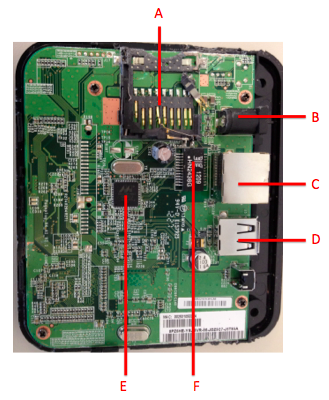
\includegraphics[width=\textwidth]{safeplug_listed_top}
  \caption{Top of the board inside the Safeplug device.}
  \label{fig:top}
\end{subfigure}%
\qquad
\begin{subfigure}[b]{.3\textwidth}
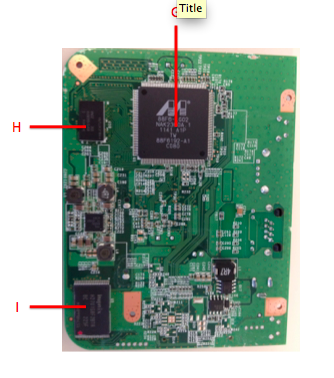
\includegraphics[width=\textwidth]{safeplug_listed_bottom}
\caption{Bottom of the board inside the Safeplug device.}
\label{fig:bottom}
\end{subfigure}
\caption{Safeplug circuit board after the teardown.}
\end{figure}


\subsection{Software}
\label{software}
We determined the software on the device from analyzing network traffic logs of the activation process (as described below) and accessing the device via SSH (as described in Section~\ref{sec:SSH}).

\subsubsection{Initial Plugin Behavior}
Before allowing the Safeplug box to be connected to the outside world, we attached it to a home connection setup formed by a computer with two network cards and then captured traffic both inside that network and between the network and the internet.  The internal network card was connected to a Netgear switch and served as a gateway, DHCP server, and DNS server.  The other card was the connection to the internet.  We used Wireshark to analyze the network data that we captured \cite{wireshark}.  

Analysis of the TCP dump showed that the Safeplug box repeatedly queried the local DNS server for two items: \url{pogoplug.com} and the NIST standardized time.  The first query for the time was to \url{www.nist.gov}, and subsequent queries included \url{nist1-chi.ustiming.org}, \url{nist1-ny.ustiming.org}, \url{time-nw.nist.gov}, and \url{nist1.symmetricom.com}.  Queries about pogoplug were mostly for \url{service.pogoplug.com} but after that set was tried \url{secure.pogoplug.com} was attempted once.  While it was only connected to the local network, we also did a scan of all the ports of the Safeplug and only port 80 was open.

\subsubsection{Activation and Update Traffic}
\label{updatetraf}
After establishing the initial update behavior, we connected the other end of our homemade router back to the internet and captured traffic on both the network interfaces. As we had seen previously, the first effort of the Safeplug was to query for \url{service.pogoplug.com} and connect, and the send a POST/XML request to that server containing a 16 byte numerical string of type \verb!nid!, \verb!0x0! as \verb!flags!, and a field called \verb!pingdata! with length of 423 bytes and undiscernable contents.  In future work, we hope to explore the contents of this automatic connection with the Pogoplug servers to discover what information is being passed along. 

The client computer then navigated to the Pogoplug website to complete the activation processes.  Each step of the process resulted in both TCP and UDP traffic between the Safeplug box and the pogoplug servers.  Most interesting was the update step in which the Safeplug box knew to request a script from \url{<update server IP>/svc/upgrade/safeplug\_switch.sh}.  Since this operation occured over normal HTTP, we were able to use \verb!curl! to recover the same script and examine it to discover the contents of the upgrade.

The upgrade script shows (and the network traffic confirms) that the box downloads and installs the following \verb!.tgz! files: 
\begin{fileName}
safeplug_lighttpd, safeplug_lighttpd_config, safeplug_wget, safeplug_certs, safeplug_gohelper, safeplug_tor, safeplug_tor_config, safeplug_privoxy, safeplug_privoxy_config
\end{fileName}
  Each file is compared to an MD5 hash before being unzipped and installed.  Details about the software found on the Safeplug are discussed in Section \ref{software}.  After the two lighttpd installations, a process called \verb!hbplug! is killed and lighttpd is started.  After the certs are downloaded, the current \verb!/usr/local/ssl! is overwritten with the new certs.  The \verb!go\_helper! is added to the \verb!/opt/xce/sbin! folder, and contains binary files with names related to update and upgrade (which we hope to decompile in future work).

After completing the installations, a default Safeplug configuation file is written with use of Tor set to 1.  (More information about the configuration in Section \ref{spconfig}.)  Finally, the old \verb!rcS! file in \verb!/etc/init.d! is replaced with commands to start lighttpd, tor and privoxy, and the LED on the front of the device is set to green after the completion of the upgrade. This means that the green LED indicates an up-to-date, internet-connected Safeplug, rather than anything about the use of TOR.

\subsubsection{Traffic After Activation}
After the activation and the configuration of the Safeplug as a proxy, all traffic was through the Tor network.  The Safeplug connected to a directory to learn about different relays and seemed to cycle through a small set around the world for different connections.  This demonstrates that Tor is working as expected.  If there is any ``phone-home'' being done by the device after Tor has been turned on, then it is doing so through the Tor network.


\subsubsection{Software on the Safeplug}
As would be suspected from the analysis of the update script described above in Section \ref{updatetraf}, the installed software is in \verb!/opt/xce! and includes lighttpd, privoxy, and tor.  Lighttpd is an open-source webserver, which is serving the settings page on the device - the project's description mentions ``security, speed, compliance, and flexibility [... while being] designed and optimized for high perfomance environments'' \cite{lighttpd}.  Privoxy is a ``non-caching web proxy with advanced filtering capabilities for enhancing privacy, modifying webpage data and HTTP headers, controlling access, and removnig ads and other obnoxious Internet junk'' and it specifically advertises its ``flexible configuration'' \cite{privoxy}.  Privoxy is also open source.  All three pieces of software appear to be there with default configuration files (with all appropriate citations and comments present).  The fourth piece of software discovered on the device, which does not seem to be installed during the activation process is the Dropbear SSH server and client, used to support SSH access to the device \cite{dropbear}.  The Safeplug uses its own configuration files to determine how these pieces of software are set up and used.
    
\subsubsection{Configuration on the Safeplug}
\label{spconfig}
The Safeplug configuration files can be found in \verb!/opt/xce/etc! and include \verb!sp.conf! and \verb!sp_version! and \verb!sp_torexceptions!.  The first contains all of the important details from the configuration page (whether to use Tor, whether to be a relay, whether to adblock) as well as a hidden option about whether to be an exitrelay for the Tor network.  This is not documented anywhere on the site, so enabling this option would likely require SSH access to discover it, thereby breaking the warranty, but it is interesting that this option is available.  The version file is likely used for updates, and the exceptions file is used by the privoxy configuation to control the whitelist of sites not to connect to via Tor.

These configuration files are read by the scripts in \verb!/opt/xce/etc/init.d! which enable lighttpd, privoxy, and tor.  As expected, Privoxy looks at the Tor, adblock and exceptions configurations, and Tor reads the \verb!sp.conf! file to set which Tor configuration file (regular, relay or exitrelay) to use.

